\problemname{Word Clock}

You work at a company producing \emph{word clocks}. These are clocks
which, instead of an ordinary clock face, have a grid of letters that
is used to display time. Inside the clock are LEDs, one behind each
letter, which are lit up in such a way that the illuminated letters
spell out the current time as a sentence. See the example below:

\begin{figure}[!h]
  \centering
  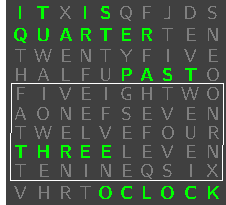
\includegraphics[scale=1.5]{wordclock.pdf}
  \begin{minipage}[c]{0.8\textwidth}
    \caption{Example word clock displaying the time 3:15. Note that for
    efficiency reasons, words are allowed to overlap, e.g. \texttt{FIVE}
    and \texttt{EIGHT}.}
  \end{minipage}
\end{figure}



Recently your company decided to go international, and you have been
tasked with designing the clock faces for various languages.
For this purpose, the team of translators has already compiled a list
of all the words needed to tell the time and arranged them into groups
according to their position in the sentence (e.g.~in the above example
the numbers from \texttt{ONE} to \texttt{TWELVE} form such a group, as
do the words \texttt{PAST} and \texttt{TO}). This means that you won't
have to worry about grammar, as you will only consider a single group
at a time.

Given such a group of words and the size of a subgrid, find a way to
place all words in the grid or determine that this is impossible.
Words have to be written from left to right and are not allowed to
wrap from one line to another.
\section*{Input}

The input consists of:
\begin{itemize}
	\item one line with three integers $h$, $w$, $n$, where
		\begin{itemize}
			\item $h$ ($1 \le h \le 18$) is the height of the grid;
			\item $w$ ($1 \le w \le 18$) is the width of the grid;
			\item $n$ ($1 \le n \le 18$) is the number of words.
		\end{itemize}
	\item one line with $n$ words, the words to fit inside the grid. 
	Each word consists of at least $1$ and at most $18$ uppercase letters of the English alphabet.
	The words are distinct.
\end{itemize}

%\begin{itemize}
%\item One line with three integers $h$, $w$, $n$ ($1 \le h,w,n \le 18$),
%	representing the height and width of the grid as well as the number of words.
%\item One line with $n$ words, the words to fit inside the grid.
%	Each word consists of at least $1$ and at most $18$ uppercase English letters.
%  The words are distinct.
%\end{itemize}

\section*{Output}

If there is no solution, print \texttt{impossible}.
Otherwise print $h$ lines, each with $w$ uppercase letters, the grid of the word clock.
If there is more than one solution, any will be accepted.

